\documentclass[__main__.tex]{subfiles}

\begin{document}

\qtitle{С}{05}
Покажите, что (а) в неоднородном электростатическом поле на диполь действует сила $\vec{F}=\left<\vec{p}_e,\nabla\right>\vec{E}$, (б) момент сил, действующий на электрический диполь в однородном электростатическом поле $\vec{E}$ равен $\vec{M}=\vec{p}_e\times\vec{E}$, где $\vec{p}_e$ -- электрический дипольный момент.\\ 
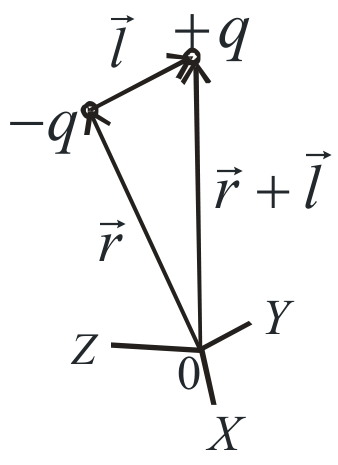
\includegraphics[scale = 0.5]{C5_1}\\
Итак, для начала запишем выражение энергии электрического диполя:\\
\begin{gather}
W = q\phi(\vec{r}+\vec{l})-q\phi(\vec{r}), \phi(\vec{r}+\vec{l}) = \phi(x+l_x,y+l_y,z+l_z)=\\
=\phi(\vec{r})+\frac{\partial \phi}{\partial x}l_x+\frac{\partial \phi}{\partial y}l_y+\frac{\partial \phi}{\partial z}+...\\
W = q\vec{l} \cdot \nabla \phi = \vec{p}_{e} \cdot (-\vec{E})
\end{gather}
Теперь мы можем выразить силу действующую на диполь:\\
\begin{gather}
\vec{F} = -\nabla W, F_i = -\frac{\partial W}{\partial x_i} = \frac{\partial}{\partial x_i}\vec{p}_{e}\vec{E}=\frac{\partial}{\partial x_i}\sum_{j=1}^{3}p_{ej}E_j = \frac{\partial}{\partial x_i} \sum_{j=1}^{3}p_{ej}\left(-\frac{\partial \phi}{\partial x_j}\right) = \\ = \sum_{j=1}^{3}\left(p_{ej}\frac{\partial}{\partial x_j}\right)\left(-\frac{\partial \phi}{\partial x_i}\right) \Longrightarrow \vec{F} = \left<\vec{p}_{e}\nabla\right>\vec{E}
\end{gather}
Момент силы, действующий на электрический диполь в однородном электростатическом поле (в однородном, значит, что $\vec{E} = const$):
\begin{gather}
\vec{M} = \vec{l} \times q\vec{E} = q\vec{l}\times\vec{E} = \vec{p}_{e}\times\vec{E}
\end{gather}
\end{document}